\section{Training Approach}

\begin{outline}
  Describe the reinforcement learning or supervised learning approach
  used to train the CNN models.
\end{outline}

\begin{figure}
  \centering
  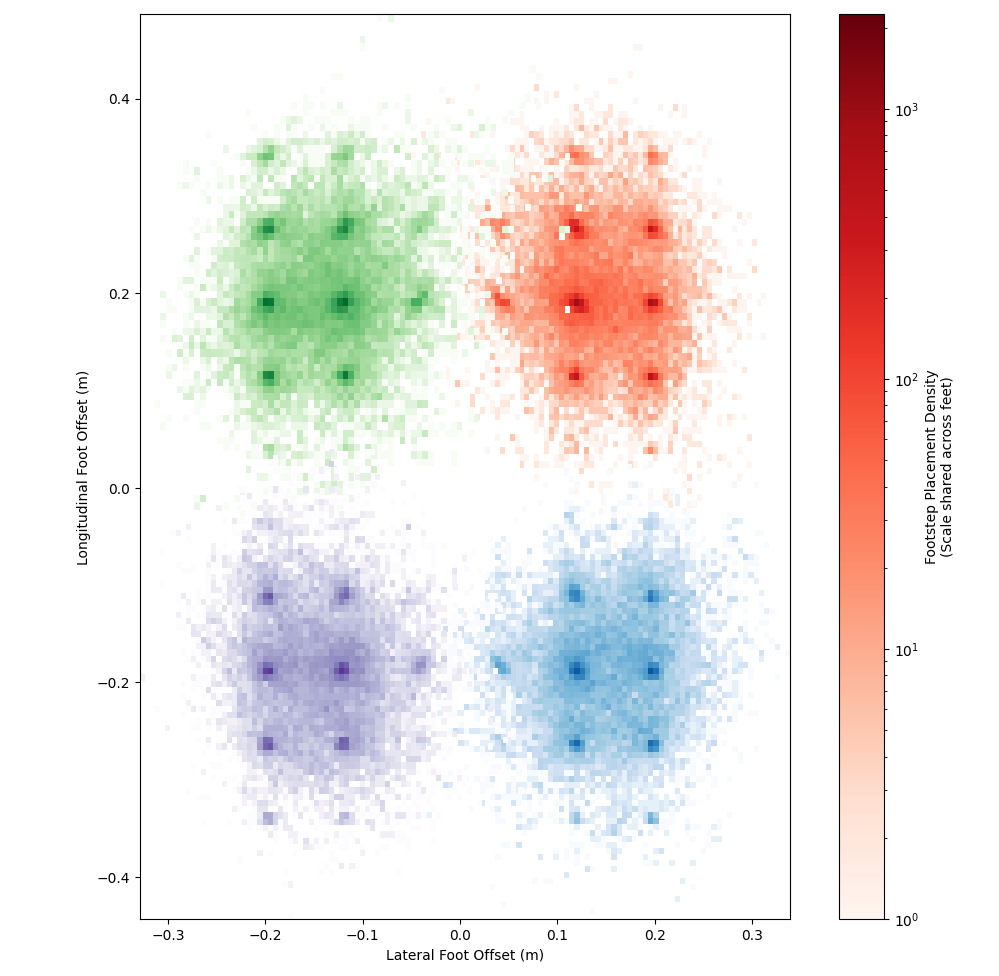
\includegraphics[width=0.8\textwidth]{images/data/foot-placement-heatmaps.png}
  \caption{Foot placement heatmaps showing distribution of foot
    positions in the GaitNet training data. Note that the histograms
  are overlaid in some places, obscuring data underneath.}
  \label{fig:data-cn-training-process}
\end{figure}

As in \cite{bratta_contactnet_2024}, the cost maps are normalized to
improve training performance. Our approach differs in how the cost
maps are normalized though. We directly normalize the cost maps to
the range $[0, 1]$, whereas \cite{bratta_contactnet_2024} normalizes
to $[0,1]$ in such a way that only the relative ordering of costs are
preserved. This difference is critical to our system to provide the
upstream GaitNet model with as much information as possible.

% \begin{figure}
%   \centering
%   \begin{minipage}[T]{0.45\textwidth}
%     \centering
%     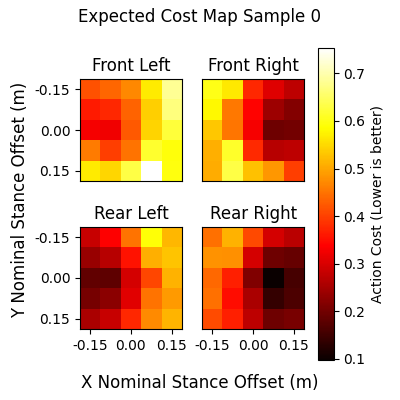
\includegraphics[width=\textwidth]{images/data/cost-map-normalization/un-normalized.png}
%   \end{minipage}
%   \hfill
%   \begin{minipage}[T]{0.45\textwidth}
%     \centering
%     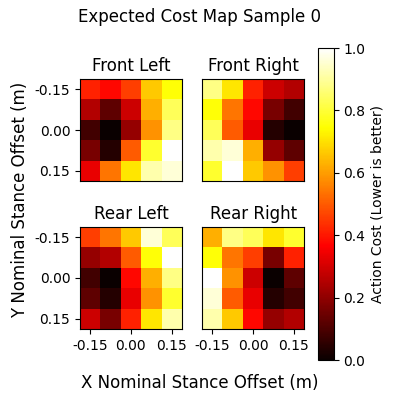
\includegraphics[width=\textwidth]{images/data/cost-map-normalization/normalized.png}
%   \end{minipage}
%   \hfill

%   \caption{Cost map normalization showing un-normalized (left) and
%   normalized (right) cost maps.}
%   \label{fig:data-cn-cost-map-normalization}
% \end{figure}

Below is the equation used as the input to the contact model.

\[
  \mathbf{x} =
  \begin{bmatrix}
    \mathbf p_{b,xy} \\
    \mathbf r_{w,z} \\
    \mathbf v_b \\
    \mathbf \omega_b \\
    \mathbf u
  \end{bmatrix}
\]

where
$\mathbf p_{b,xy}$ is the $x$ and $y$ position all end effectors in
the base frame stacked into a single vector,
$\mathbf r_{w,z}$ is the height of the robot's COM in the world frame.

The model is trained on $y$, the heuristically calculated footstep
cost maps (\autoref{fig:data-footstep-cost-map}).

\begin{figure}
  \centering
  \includegraphics[width=0.75\linewidth]{images/data/footstep-cost-map.png}
  \caption{Footstep cost map. Shows the heuristic cost for each
  possible footstep location.}
  \label{fig:data-footstep-cost-map}
\end{figure}

Here, the inclusion of $\mathbf \omega_b$ differs from
\cite{bratta_contactnet_2024}

The results of this model are very promising, with the model able to
predict footstep cost maps with high accuracy.
\autoref{fig:data-cn-typical-comparison}
shows the model output and ground truth for typical data sample.
\autoref{fig:data-cn-challenging-comparison}
shows a particularly challenging data sample, and the model is still
able to identify the best positions for each leg,
particularly the back left leg, which needs to be far from the
nominal position to maintain stability in that state.

\begin{figure}
  \centering
  \begin{minipage}[T]{0.45\textwidth}
    \centering
    \includegraphics[width=\textwidth]{images/data/training/typical-expected.png}
  \end{minipage}
  \hfill
  \begin{minipage}[T]{0.45\textwidth}
    \centering
    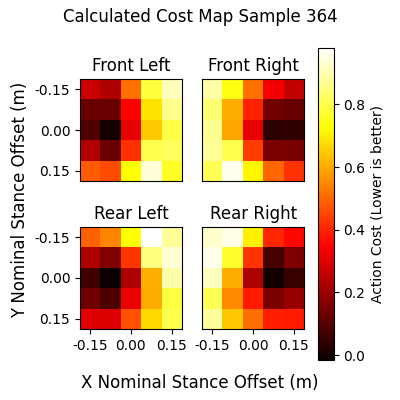
\includegraphics[width=\textwidth]{images/data/training/typical-calculated.png}
  \end{minipage}
  \hfill

  \caption{Typical data samples showing calculated (left) and
  expected (right) quadruped images.}
  \label{fig:data-cn-typical-comparison}
\end{figure}

\begin{figure}
  \centering
  \begin{minipage}[T]{0.45\textwidth}
    \centering
    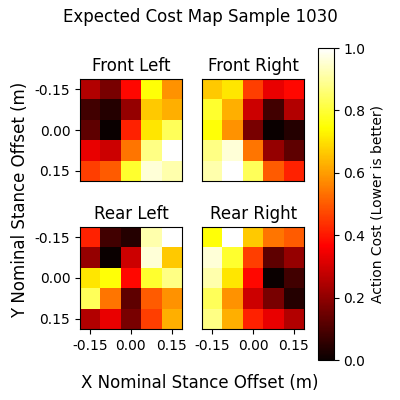
\includegraphics[width=\textwidth]{images/data/training/challenging-expected.png}
  \end{minipage}
  \hfill
  \begin{minipage}[T]{0.45\textwidth}
    \centering
    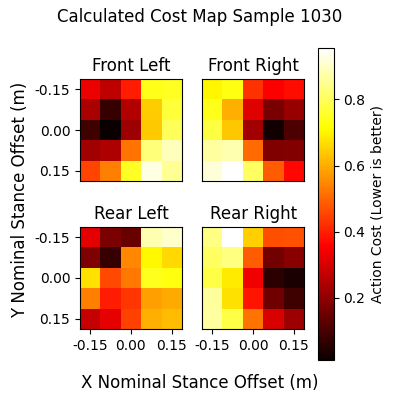
\includegraphics[width=\textwidth]{images/data/training/challenging-calculated.png}
  \end{minipage}
  \hfill

  \caption{Particularly challenging data samples showing calculated (left) and
  expected (right) quadruped images.}
  \label{fig:data-cn-challenging-comparison}
\end{figure}
